
% This LaTeX was auto-generated from MATLAB code.
% To make changes, update the MATLAB code and republish this document.

\documentclass{article}
\usepackage{graphicx}
\usepackage{color}

\sloppy
\definecolor{lightgray}{gray}{0.5}
\setlength{\parindent}{0pt}

\begin{document}

    
    
\subsection*{Contents}

\begin{itemize}
\setlength{\itemsep}{-1ex}
   \item COMPILATION
   \item SIMULATION
   \item ODE15S
   \item PLOTTING
   \item FORWARD SENSITIVITY ANALYSIS
   \item FINITE DIFFERENCES
   \item PLOTTING
\end{itemize}
\begin{verbatim}
clear
\end{verbatim}


\subsection*{COMPILATION}

\begin{verbatim}
[exdir,~,~]=fileparts(which('example_model_2.m'));
% compile the model
amiwrap('model_example_2','example_model_2_syms',exdir)
\end{verbatim}

        \color{lightgray} \begin{verbatim}Generating model struct ...
Parsing model struct ...

Generating C code ...
headers | wrapfunctions | 
Compiling mex file ...
Building with 'Xcode with Clang'.
MEX completed successfully.
\end{verbatim} \color{black}
    

\subsection*{SIMULATION}

\begin{verbatim}
% time vector
t = linspace(0,3,1001);
p = [1;0.5;2;3];
k = [];

options.sensi = 0;
options.cvode_maxsteps = 1e6;
% load mex into memory
[msg] = which('simulate_model_example_2'); % fix for inaccessability problems
sol = simulate_model_example_2(t,log10(p),k,[],options);

tic
sol = simulate_model_example_2(t,log10(p),k,[],options);
disp(['Time elapsed with amiwrap: ' num2str(toc) ])
\end{verbatim}

        \color{lightgray} \begin{verbatim}Time elapsed with amiwrap: 0.0029045
\end{verbatim} \color{black}
    

\subsection*{ODE15S}

\begin{verbatim}
sig = 1e-2;
delta_num = @(tau) exp(-1/2*(tau/sig).^2)/(sqrt(2*pi)*sig);

ode_system = @(t,x,p,k) [-p(1)*x(1)+delta_num(t-p(2));
    +p(3)*x(1) - p(4)*x(2)];

options_ode45 = odeset('RelTol',1e-8,'AbsTol',1e-8,'MaxStep',1e4);

tic
[~, X_ode45] = ode45(@(t,x) ode_system(t,x,p,k),t,[0;0],options_ode45);
disp(['Time elapsed with ode45: ' num2str(toc) ])
\end{verbatim}

        \color{lightgray} \begin{verbatim}Time elapsed with ode45: 0.065563
\end{verbatim} \color{black}
    

\subsection*{PLOTTING}

\begin{verbatim}
figure
c_x = get(gca,'ColorOrder');
subplot(2,2,1)
for ix = 1:size(sol.x,2)
    plot(t,sol.x(:,ix),'.-','Color',c_x(ix,:))
    hold on
    plot(t,X_ode45(:,ix),'--','Color',c_x(ix,:))
end

legend('x1','x1_{ode45}','x2','x2_{ode15s}','Location','NorthEastOutside')
legend boxoff
xlabel('time t')
ylabel('x')
box on
subplot(2,2,2)
plot(t,abs(sol.x-X_ode45),'--')
set(gca,'YScale','log')
ylim([1e-10,1e0])
legend('error x1','error x2','Location','NorthEastOutside')
legend boxoff

subplot(2,2,3)
plot(t,sol.y,'.-','Color',c_x(1,:))
hold on
plot(t,X_ode45(:,2),'--','Color',c_x(1,:))
legend('y1','y1_{ode45}','Location','NorthEastOutside')
legend boxoff
xlabel('time t')
ylabel('y')
box on

subplot(2,2,4)
plot(t,abs(sol.y-X_ode45(:,2)),'--')
set(gca,'YScale','log')
ylim([1e-10,1e0])
legend('error y1','Location','NorthEastOutside')
legend boxoff
xlabel('time t')
ylabel('y')
box on
set(gcf,'Position',[100 300 1200 500])
\end{verbatim}

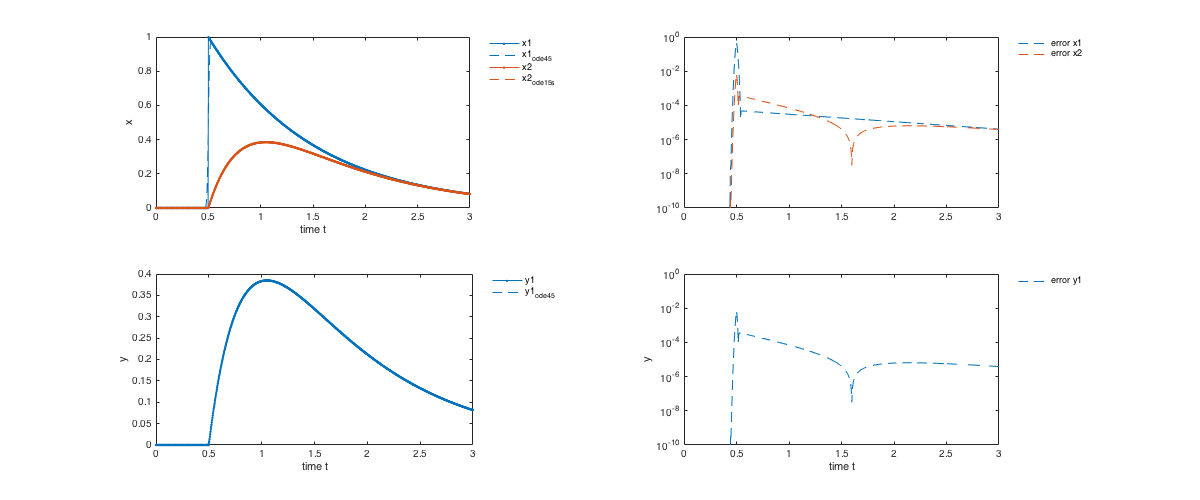
\includegraphics [width=4in]{example_model_2_01.png}


\subsection*{FORWARD SENSITIVITY ANALYSIS}

\begin{verbatim}
options.sensi = 1;

sol = simulate_model_example_2(t,log10(p),k,[],options);
\end{verbatim}


\subsection*{FINITE DIFFERENCES}

\begin{verbatim}
eps = 1e-4;
xi = log10(p);
for ip = 1:4;
    xip = xi;
    xip(ip) = xip(ip) + eps;
    solp = simulate_model_example_2(t,xip,k,[],options);
    sx_fd(:,:,ip) = (solp.x - sol.x)/eps;
    sy_fd(:,:,ip) = (solp.y - sol.y)/eps;
end
\end{verbatim}


\subsection*{PLOTTING}

\begin{verbatim}
figure
for ip = 1:4
    subplot(4,2,ip*2-1)
    hold on
    for ix = 1:size(sol.x,2)
        plot(t,sol.sx(:,ix,ip),'.-','Color',c_x(ix,:))
        plot(t,sx_fd(:,ix,ip),'--','Color',c_x(ix,:))
    end
    ylim([-2,2])
    legend('x1','x1_{fd}','x2','x2_{fd}','Location','NorthEastOutside')
    legend boxoff
    title(['state sensitivity for p' num2str(ip)])
    xlabel('time t')
    ylabel('x')
    box on

    subplot(4,2,ip*2)
    plot(t,abs(sol.sx(:,:,ip)-sx_fd(:,:,ip)),'r--')
    legend('error x1','error x2','Location','NorthEastOutside')
    legend boxoff
    title(['state sensitivity for p' num2str(ip)])
    xlabel('time t')
    ylabel('error')
    ylim([1e-12,1e0])
    set(gca,'YScale','log')
    box on
end
set(gcf,'Position',[100 300 1200 500])

figure
for ip = 1:4
    subplot(4,2,ip*2-1)
    hold on
    for iy = 1:size(sol.y,2)
        plot(t,sol.sy(:,iy,ip),'.-','Color',c_x(iy,:))
        plot(t,sy_fd(:,iy,ip),'--','Color',c_x(iy,:))
    end
    ylim([-2,2])
    legend('y1','y1_{fd}','Location','NorthEastOutside')
    legend boxoff
    title(['observable sensitivity for p' num2str(ip)])
    xlabel('time t')
    ylabel('y')
    box on

    subplot(4,2,ip*2)
    plot(t,abs(sol.sy(:,:,ip)-sy_fd(:,:,ip)),'r--')
    legend('error y1','Location','NorthEastOutside')
    legend boxoff
    title(['observable sensitivity for p' num2str(ip)])
    xlabel('time t')
    ylabel('error')
    ylim([1e-12,1e0])
    set(gca,'YScale','log')
    box on
end
set(gcf,'Position',[100 300 1200 500])
\end{verbatim}

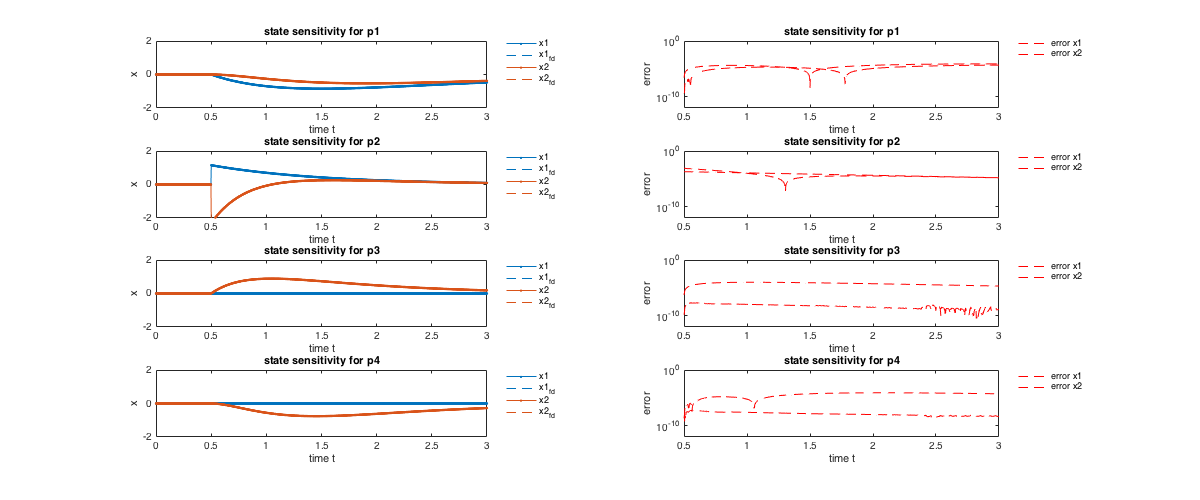
\includegraphics [width=4in]{example_model_2_02.png}

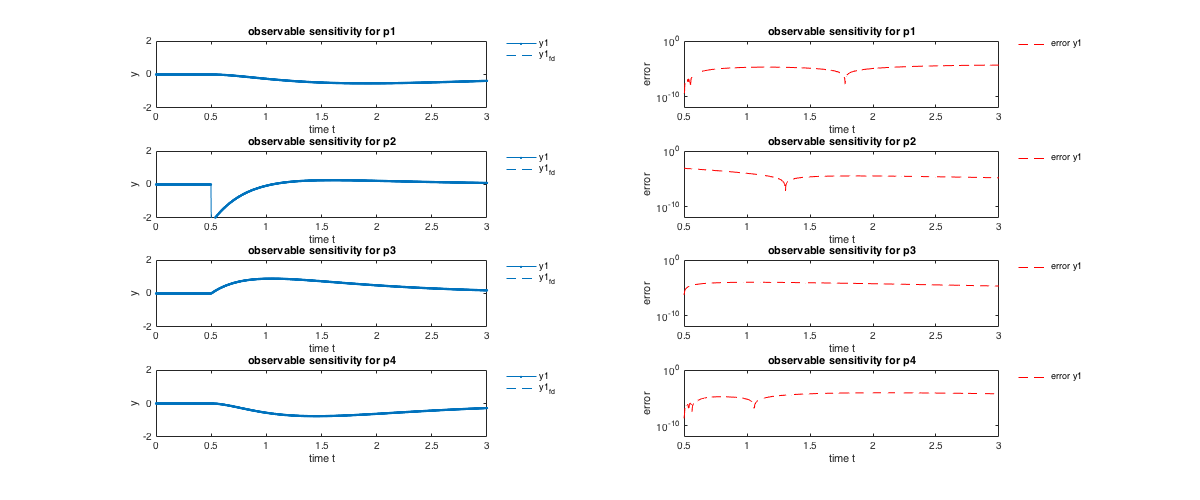
\includegraphics [width=4in]{example_model_2_03.png}



\end{document}
    
